% Converted from reference/DB4OTutorial (MadCap Flare, Java target)

\chapter{Activation}
\label{tut:activation}

Activation is a mechanism which controls object instantiation. Why is this necessary? Let's look at an example. We store person-objects with its parents. Each person object has a reference to his parents, the parents again have references to their parents and so on and so forth. Now we load a person object from the database, what does db4o do? Does it load the person object, its parents and the parents of the parents? Then it probably loads all objects from the database and will use up all memory.

\begin{center}
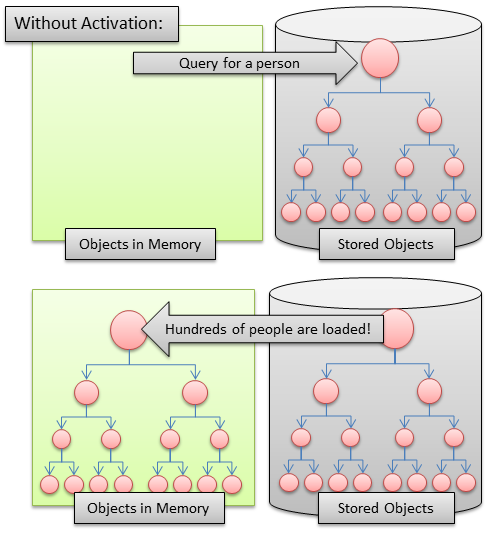
\includegraphics[width=\maxwidth]{images/tut-without-activation.png}
\end{center}
Luckily db4o does not behave like this. When a query retrieves objects, their fields are loaded into memory (activated in db4o terms) only to a certain activation depth. In this case depth means "number of member references away from the original object". All the fields beyond the activation depth are set to null or to default values.So db4o does not load the whole object graph at once. Instead, db4o loads only the parts which we are interested in.

\begin{center}
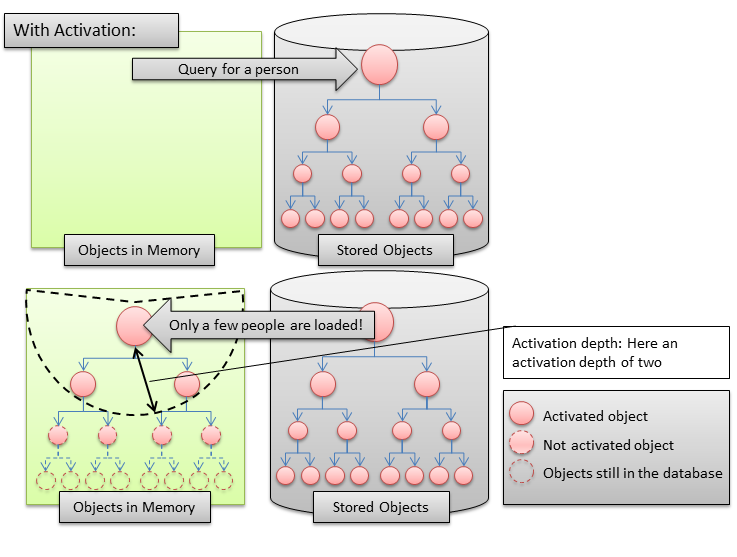
\includegraphics[width=\maxwidth]{images/tut-with-activation.png}
\end{center}
\section{Activation in Action}
\label{tut:activation:activationinaction}

Let's see db4o's activation in action. To do so we need a deep object-graph. We create a person class with a mother-field and then create a deep hierarchy of people, for example a hierarchy of seven people.

\begin{lstlisting}
public class Person {
    private String name;
    private Person mother;

    public Person(String name, Person mother) {
        this.name = name;
        this.mother = mother;
    }

    public String getName() {
        return name;
    }

    public Person getMother() {
        return mother;
    }

    @Override
    public String toString() {
        return "Person{" +
                "name='" + name +
                "'}";
    }
}
\end{lstlisting}

{\small\itshape Person.java: Domain model for people\par}
\medskip

\begin{lstlisting}
Person eva = new Person("Eva",null);
Person julia = new Person("Julia",eva);
Person jennifer = new Person("Jennifer",julia);
Person jamie = new Person("Jamie",jennifer);
Person jill = new Person("Jill",jamie);
Person joanna = new Person("Joanna",jill);

Person joelle = new Person("Joelle",joanna);
container.store(joelle);
\end{lstlisting}

{\small\itshape ActivationConcept.java: Store a deep object hierarchy\par}
\medskip

After that we close the database, reopen it and query for a person. Then we start to traverse the object graph. At a certain point we will reach objects which aren't activated anymore. In those objects all fields are null or have the default value:

\begin{lstlisting}
Person joelle = queryForJoelle(container);
Person jennifer = joelle.getMother().getMother().getMother().getMother();
System.out.println("Is activated: " + jennifer);
// Now we step across the activation boundary
// therefore the next person isn't activate anymore.
// That means all fields are set to null or default-value
Person julia = jennifer.getMother();
System.out.println("Isn't activated anymore"+julia);
\end{lstlisting}

{\small\itshape ActivationConcept.java: Activation depth in action\par}
\medskip

Since not activate objects have set all their fields to null, they can cause null pointer exceptions:

\begin{lstlisting}
String nameOfMother = julia.getMother().getName();
\end{lstlisting}

{\small\itshape ActivationConcept.java: NullPointer exception due to not activated objects\par}
\medskip

\section{Deal With Activation}
\label{tut:activation:dealwithactivation}

We've seen that activation can cause issues and we have to deal with it. There are different strategies for that.

\subsection*{Directly Activating Objects}

We can explicitly activate objects or ask about their activation state. This way we can activate objects when needed. However as soon as we need to activate objects explicitly all over the place in our code we should look for alternatives.

\begin{lstlisting}
boolean isActivated = container.ext().isActive(julia);
\end{lstlisting}

{\small\itshape ActivationConcept.java: Check if an instance is activated\par}
\medskip

\begin{lstlisting}
container.activate(julia,5);
\end{lstlisting}

{\small\itshape ActivationConcept.java: Activate instance to a depth of five\par}
\medskip

\subsection*{Changing Activation Depth}

Alternatively we can increase the activation depth globally or for certain types. However we need to be aware that a high activation depth decreases performance. That's why we should be very careful with increasing the activation depth.

\begin{lstlisting}
EmbeddedConfiguration configuration = Db4oEmbedded.newConfiguration();
configuration.common().activationDepth(10);
ObjectContainer container = Db4oEmbedded.openFile(configuration,DATABASE_FILE);
\end{lstlisting}

{\small\itshape ActivationConcept.java: Increase the activation depth to 10\par}
\medskip

We can even more fine tune the activation depth. However the fundamental issue is the same. When we increase the activation depth it will hurt performance.

\begin{lstlisting}
EmbeddedConfiguration configuration = Db4oEmbedded.newConfiguration();
// At least activate persons to a depth of 10
configuration.common().objectClass(Person.class).minimumActivationDepth(10);
// Or maybe we just want to activate all referenced objects
configuration.common().objectClass(Person.class).cascadeOnActivate(true);
\end{lstlisting}

{\small\itshape ActivationConcept.java: More activation options\par}
\medskip

\subsection*{Transparent Activation / Persistence}

The last option we have is transparent activation. Transparent activation takes care of all activation issues. It activates objects as soon as they are needed. To get transparent activation we need to enhance our classes at compile time. Read \hyperref[tut:transparentpersistence]{this section of the tutorial} (p.~\pageref{tut:transparentpersistence}) where we use transparent activation.

